\chapter{Interface between KKMC-hh and MG5\textunderscore aMC@NLO}
With the help of KKMC-hh \cite{KKMC-hh1,KKMC-hh2,KKMC0hh3}, the coherent exclusive exponentiation (CEEX) electroweak (EW) exact $O(\alpha^2L)$ correction for the Drell-Yan process (please read Appendix E) has been achieved. In order to realize the EW+the next-to-leading order (NLO) QCD correction for the Drell-Yan process, we will first apply the Madgraph5\textunderscore aMC@NLO (MG5\textunderscore aMC@NLO) \cite{MG5} to obtain the next-to-leading order QCD correction, and then we will interface KKMC-hh with MG5\textunderscore aMC@NLO via merging their LHE files to achieve the EW and NLO QCD corrections. In this chapter, we will first introduce the overview of MG5\textunderscore aMC@NLO. Next we will describe the approach to interface KKMC-hh with MG5\textunderscore aMC@NLO. Finally we will exhibit and discuss our results. 

\section{Overview of Madgraph\textunderscore aMC@NLO}

MADGRAPH \cite{madgraph} is a powerful tool for automatically generating matrix elements for high energy physics process, such as $2\to n$ scatterings and decays. First the user inputs a specific process in terms of initial and final particles, allowing some refined criteria. As a result, MADGRAPH generates all Feynman diagrams for the process, and yields the computer code to compute the matrix element at a given phase space point. The matrix element calculation is done using the helicity amplitudes technique which was first implemented in the package HELAS \cite{helas}. The application of the helicity amplitudes is efficient because it allows the helicity amplitudes corresponding to identical subdiagrams to be reused between the diagrams, leading a considerable optimization. The computer code generate by MADGRAPH can then be used for the cross section and decay width evaluation and event generation.

 The essential idea of MADGRAPH5\textunderscore aMC@NLO is the same as the MADGRAPH family. The structure of a cross section is essentially independent of the process regardless of the theory and of the perturbative order, and thus it can be written as a computer code once and for all. For example, phase phases can be defined in full generality, leaving only particle masses and number as free parameters. Conversely, matrix elements which are obviously dependent on the theory and process can be calculated starting from a limited number of formal instructions, such as Feynman rules and recursion relations. 
 MADGRAPH5\textunderscore aMC@NLO is written in a meta-code, in which a Python code writes a Python, C++ or Fortan code. The latter code is specific to the desired process. MADGRAPH5\textunderscore aMC@NLO includes two ingredients. The first one is a theory model, which is equivalent to the Lagrangian of the theory and its parameters, such as masses and coupling constant. The second one is a set of process-indepedent building blocks for automation of calculations. The automation of NLO computation  
 involves the FKS subtraction block, which carrys out the generation of the real corrections with the proper subtractions automatically \cite{fks1,fks2,fks3,fks4,fks5,fks6}, by interfacing MadFKS \cite{fks6}. Besides the module for real corrections, the automation of NLO computation requires a specific module for virtual corrections. In MG5\textunderscore aMC@NLO, the virtual contribution to an NLO cross section is achieved through the module MADLOOP \cite{madloop}, which is based on the OPP integrand reduction technique \cite{opp}. These two module above together allow a fully automatic computation of infrared-safe observables at NLO in QCD. After the integration of the matrix element hard process,  the full parton shower and hadronization infrastructures, such as Herwig and Pythia, etc., are also critical for an accurate simulation of a hadronic process. In this thesis, we have applied MG5\textunderscore aMC@NLO + Herwig to obtain the simulation of the Drell-Yan process $pp\to Z/\gamma\to \mu^+\mu^-+X$ at the nex-to-leading order in QCD.
 
\newpage 
 \section{Interfacing KKMC-hh with MG5\textunderscore aMC@NLO}
We will now introduce our approach to interface KKMC-hh and MG5\textunderscore aMC@NLO. Our essential idea is 
merging their LHE \cite{LHE} files to achieve the EW and NLO QCD corrections. Namely, given that LHE file from the MG5\textunderscore aMC@NLO contains all the information of the events at the partonic level, we extract the next-to-leading order contribution in QCD for Drell-Yan process from the LHE file and combine it with the weight of KKMC-hh to achieve the EW and NLO QCD corrections of the Drell-Yan process. We are exhibiting our method in details in the following.
 
In the KKMC-hh, the basic event $(x_1,x_2,v,W_\text{Basic})$ is generated by the distribution
 \begin{align}
 \rho =&  2N_q  [\frac{Q_s^2}{z^2s}(\frac{1}{Q_{smin}}-\frac{1}{Q_{samx}})]log(\frac{s}{Q_s})f_{q_1}(\sqrt{Q_s},x_1)f_{\bar{q}_2}(\sqrt{Q_s},x_2)\nonumber\\&\times \frac{1}{2} (\frac{\bar{\gamma}}{
 	\gamma}) (\frac{v}{v_{min}})^{\bar{\gamma}-\gamma} (1+\frac{1}{\sqrt{1-v}})v_{max}^{\gamma}\nonumber\\
 &\times\frac{ \sigma_{Born}((1-v)Q_s)}{3(1-v)}.
 \end{align}
 which includes three components: 
\begin{align*}
 \rho(x_1,x_2)&=2N_q  [\frac{Q_s^2}{z^2s}(\frac{1}{Q_{smin}}-\frac{1}{Q_{samx}})]log(\frac{s}{Q_s})f_{q_1}(\sqrt{Q_s},x_1)f_{\bar{q}_2}(\sqrt{Q_s},x_2),\nonumber\\
 \rho(v)&=\frac{1}{2} (\frac{\bar{\gamma}}{
 	\gamma}) (\frac{v}{v_{min}})^{\bar{\gamma}-\gamma} (1+\frac{1}{\sqrt{1-v}})v_{max}^{\gamma},\text{ and }
\frac{ \sigma_{Born}((1-v)Q_s)}{3(1-v)},
\end{align*} 
where $x_1$ and $x_2$ describe beamstrahlung, $v$ describes the total energy loss due to ISR, and $W_\text{Basic}$ is the weight corresponding to the basic event.



 The weight \textbf{XWGTUP} derived from the LHE file of MG5\textunderscore aMC@NLO repesents the cross section of the process in units of pb, which includes the partonic cross section, contributions from parton distribution functions (PDF) and the perturbative QCD corrections. To be more specific,
 for the Drell-Yan process $pp\rightarrow Z/\gamma^\ast\rightarrow l^+ l^-+X$, the differential cross section is
 \begin{equation}
 \frac{d\sigma}{dy dM}=\sum_{i,j}^{}\hat{\sigma}_{Born}\int_{x_1}^{1} dx_i\int_{x_2}^{1} dx_j f_i(x_i,Q^2) f_j(x_j,Q^2) \Delta(x_1,x_2,x_i,x_j,Q^2)
 \end{equation}
 where $\hat{\sigma}_{Born}$ is s the partonic cross section of the Drell-Yan process, $\Delta_{ij}$ is the
 perturbative QCD coefficient function for the Drell-Yan process. And the partonic cross section of the Drell-Yan process can be written as
 \begin{equation}
 \hat{\sigma}_{Born} = \frac{1}{3} \cdot \frac{4\pi\alpha^2}{3Q^2}\sum q_f^2.
 \end{equation}
 
 In order to interface MG5\textunderscore aMC@NLO with KKMC-hh, we need to replace the basic weight $W_\text{Basic}$ with the weight from \textbf{XWGTUP} after removing the intersections between $W_\text{Basic}$ and \textbf{XWGTUP}, and use momentums of intial quark paris derived from LHE file of MG5\textunderscore aMC@NLO to generate a new pair of parton momentum fractions $x_1$ and $x_2$.
 
 We see \textbf{XWGTUP} has three components: partonic cross section $\hat{\sigma}_{Born}$, the function of $x_i$ and $x_j$ and QCD corrections. So the intersections between $W_\text{Basic}$ and \textbf{XWGTUP} are $\hat{\sigma}_{Born}$ and the function of $x_1$ and $x_2$. Therefore,  we need to remove $\rho(x_1,x_2)$  from $\rho$. Since KKMC-hh would calculate the crude Born cross section after ISR generation, we remove $\hat{\sigma}_{Born}$ from $XWGTUP$. Then, we could have the $\rho'$
 \begin{equation}
 \rho' = \frac{XWGTUP}{\hat{\sigma}_{Born}} \times \frac{1}{2} (\frac{\bar{\gamma}}{
 	\gamma}) (\frac{v}{v_{min}})^{\bar{\gamma}-\gamma} (1+\frac{1}{\sqrt{1-v}})v_{max}^{\gamma} \frac{ \sigma_{Born}((1-v)Q_s)}{3(1-v)}
 \end{equation} 
 
 In $\rho(x_1,x_2)$, the factor $2N_q$ comes from summation over quarks, where $N_q$ is determined by the subroutine \textbf{hh\textunderscore Quarks}. Since we need to replace $\rho(x_1,x_2)$ with the \textbf{LHE} weight removing the Born cross section calculated by MG5\textunderscore aMC@NLO, $\textbf{XWGTUP}/\hat{\sigma}_{Born}$, we would replace this factor together with $\rho(x_1,x_2)$ in the program.
 
 In order to realize our approach in the computer programming, we first coded a new subroutine \textbf{UPYVNT}, which read event information from the LHE file of MG5\textunderscore aMC@NLO. Then we coded another new subroutine  \textbf{hh\textunderscore MakeLHE} (called before the subroutine \textbf{hhFoam\textunderscore Make}) to use momentums $\hat{p_1}$ and $\hat{p_2}$ of initial quark pairs from LHE file to compute the pair of $x_1$ and $x_2$ as follows:
\begin{align}
&Q_s =Q^2 = (\hat{p}_1+\hat{p}_2)^2,\nonumber\\
&z=\frac{Qs}{s}, 
 \end{align}
where $s=E_\text{CMS}^2$. Then we have
 $$
 x_1 = z^{r_2}, x_2 = z^{1-r_2},
 $$
 where $r_2$ is a random number. And the corresponding weight is
 $$
W_\text{LHE} = \frac{\textbf{XWGTUP}}{\hat{\sigma}_\text{Born}}.
 $$
 Ater generating $x_1$ and $x_2$, we modified the subroutine \textbf{hhBornV\textunderscore RhoFoam} so that it would only calculate $\bar{\gamma}$ and $\gamma$ with the help of new $Q_s$ and generate a new $v$. In sum, the new $W_\text{Basic}$ is calculated according to eq. (8.4). 
 
 With the help of the new basic weight of eq. (8.4), the cross section for interfacing KKMC-hh with MG5\textunderscore aMC@NLO can be evaluated by 
 \begin{equation}
 \sigma = \rho'<\prod_{k} w_k>.
 \end{equation}
 In the program, this cross section is calculated by the average of main weight $W_\text{Main}$. The main  weight has two components $W_\text{Crud}$ and $W_\text{Best}$:
 \begin{equation*}
W_\text{Main} = W_\text{Crud} \times W_\text{Best}.
 \end{equation*} 
 The crude weight $W_\text{Crud}$ is calculated in subroutine \textbf{KK2f\textunderscore Make}. The crude weight has two components, the ISR components $W_\text{ISR}$  and the FSR components $W_\text{FSR}$.
 
 \begin{equation*}
W_\text{Crud} =W_\text{ISR}  \times W_\text{FSR} ,
 \end{equation*}
 where the ISR components $W_\text{ISR}$ is calculated by subroutine \textbf{KarLud\textunderscore Make} and the FSR components $W_\text{FSR}$ is calculated by subroutine \textbf{KarFin\textunderscore Make}
 \begin{align*}
W_\text{ISR} = W_\text{Basic} \times W_\text{Mass} \times W_\text{Dil} \times W_\text{Cut} \times  W_\text{KF},
 \end{align*}
 
 \begin{equation}
{W_\text{FSR}} = W_1 \times W_2 \times W_3,
 \end{equation}
 
 The brief explanations for components are as follows:

 (\romannumeral 1) $W_\text{Basic}$: the basic weight $W_\text{Basic}$ is calculated by eq. (8.4), which generates $v$, $x_1$ and $x_2$. It includes not only the electroweak contribution but the NLO QCD corrections as well.

  (\romannumeral 2) $W_\text{Mass}$: the weight $W_\text{Mass}$ corresponds the simplification made on the photon angular distribution by dropping mass terms. If there is no photon above detectablity threshold, then
 \begin{equation*}
 W_\text{Mass} = 1.
 \end{equation*}
 If not, 
 \begin{eqnarray}
W_\text{Mass} = \prod_{i=1}^{n}\frac{f(\theta_i)}{\bar{f}(\theta_i)}.
 \end{eqnarray} 
 where
\begin{align}
f(\theta_i)& = \frac{\alpha}{\pi^2}\biggl[\frac{1}{(1-\beta cos\theta_i)(1+\beta cos\theta_i)}-\frac{m_e^2}{s}\frac{1}{(1-\beta cos\theta_i)^2}-\frac{m_e^2}{s}\frac{1}{(1+\beta cos\theta_i)^2}\biggr],\nonumber\\
\bar{f}(\theta_i) &= \frac{\alpha}{\pi^2}\frac{1}{(1-\beta cos\theta_i)(1+\beta cos\theta_i)}.
\end{align}

  (\romannumeral 3) $W_\text{Dil}$: this weight corresponds to the simplification made on the dilatation Jacobian.

\begin{align}
 J(\bar{k},v)=\frac{1}{2}\left(1+\frac{1}{\sqrt {1-Av}}\right) \longrightarrow
 J_0(v)=\frac{1}{2}\left(1+\frac{1}{\sqrt{1-v}}\right).
\end{align}
We therefore have
 \begin{equation}
 W_\text{Dil}=\frac{J(\bar{k},v)}{J_0(v)}=\frac{1+\sqrt{1-Av}}{1+\sqrt{1-v}}.
 \end{equation}


   (\romannumeral 4) $W_\text{Cut}$: this weight corresponds to the lower photon energy boundary:
 \begin{equation}
 W_\text{Cut} = \theta\left(\lambda_0(\bar{k},v)x_n-\epsilon\right)=  \theta\left(\frac{2k^n_0}{\sqrt{s}}-\varepsilon\right).
 \end{equation}
 
  (\romannumeral 5) $W_\text{KF}$: this weight corresponds the generation of \textbf{KF} codes, generated by subroutine \textbf{MBrA\textunderscore GenKF}.

 (\romannumeral 6) $W_1$: it is the weight corresponding to phase space limits for very hard photon, generated by subroutine \textbf{KarFin\textunderscore YFSfin},
 \begin{equation}
 W_1 = 1.
 \end{equation}

  (\romannumeral 7) $W_2$: it corresponds to the weight for translation Jacobian, generated by subroutine \textbf{KarFin\textunderscore YFSfin},
 \begin{equation}
 W_2=\frac{1+\bar{K}^0}{1+\bar{K}^0+\frac{1}{4}\bar{K}^2}.
 \end{equation}


 (\romannumeral 7) $W_3$: it is the weight that corresponds to the following simplifiications: 

\begin{align}
 f \left(\theta_j,\frac{m^2_f}{s_Q}\right) \longrightarrow \bar{f}\left(\theta_j,\frac{m^2_f}{s_X}\right), \quad e^{\gamma_f \log(\delta_f((1+\bar{K}^0)))} \longrightarrow e^{\gamma_f \log (\delta_f)}
\end{align}
where
\begin{align}
 f(\theta_j,\frac{m^2_f}{s_Q})&=\frac{1+\beta_f^2}{\delta_{1j}\delta_{2j}}-\frac{\mu_f^2}{2}\frac{1}{\delta_{1j}^2}-\frac{\mu_f^2}{2}\frac{1}{\delta_{2j}^2},\nonumber\\
 \delta_{1j}&=1-\beta_f cos\theta_j,\nonumber\\
 \delta_{2j}&=1+\beta_f cos\theta_j,\nonumber\\
  \bar{f}(\theta_j,\frac{m_f^2}{s_X})&=\frac{1+\bar{\beta}_f^2}{\bar{\beta}_f^2}\frac{1}{1-\bar{\beta}_f^2 cos^2\theta_j}.\nonumber\\
  \bar{\beta_f}&=\sqrt{1-\left(\frac{m_f^2}{s_X}\right)^2},\nonumber\\
  \bar{\gamma_f}&=Q_f^2 \frac{\alpha}{\pi} \frac{1+\bar{\beta_f}^2}{\bar{\beta_f}}\log\frac{1+\bar{\beta}_f}{1-\bar{\beta}_f}.
\end{align}
Therefore, we have
 \begin{equation}
 W_3=e^{\gamma_f \log(\delta_f((1+\bar{K}^0)))-\gamma_f \log (\delta_f)}\prod_{j=1}^{n'}\frac{f\left(\theta_j,\frac{m_f^2}{s_Q}\right)}{\bar{f}\left(\theta_j,\frac{m_f^2}{s_X}\right)}
 \end{equation}

 And the model weight weight $W_\text{Best}$ is of the $O(\alpha^{(2)})$, calculated by the subroutine \textbf{GPS\textunderscore Make},
\begin{equation}
W^{(2)}_\text{CEEX}(p_a,p_b,p_c,p_d;k_1,\ldots,k_{n})=\frac{\rho^{(2)}_\text{CEEX}(p_a,p_b,p_c,p_d;k_1,\ldots,k_{n})}{\rho_{[\dot{n},n']}^\text{Cru}(p_c,p_d;k_1,\ldots,k_{n})(2\pi)^{3(n+2)-4}}.
\end{equation}
 Please read Section (7.2) and Subsection (7.4.1) for details.
 
 Therefore, with the help of the $W_\text{Main}$, the cross section which includes electroweak and NLO QCD corrections will be evaluated. Our results will be exhibited in the next section.
 
\section{Numerical Results for Interfacing KKMC-hh with MG5\textunderscore aMC@NLO} 
 
We will now discuss the results of interfacing KKMC-hh with MG5\textunderscore aMC@NLO. Specifically, we compared the results of the Drell-Yan process $pp\to Z/\gamma^\ast\to \mu^+\mu^-+X$ obtained by KKMC-hh, MG5\textunderscore aMC@NLO and MG5\textunderscore aMC@NLO interfaced with KKMC-hh respectively. We made these comparisons at $\sqrt{s}=13 \text{ TeV}$ with the ATLAS cuts on the $Z/\gamma^\ast$ production and decay to lepton pairs \cite{ATLAS}:
\begin{equation*}
80 \text{ GeV} < M_{\ell\ell}<100 \text{ GeV},\qquad P^{\ell\ell}_T<30\text{ GeV}
\end{equation*}
where both memebers of the decay lepton pair satisfy 
\begin{equation*}
P^{\ell}_T>25\text{ GeV},\qquad |\eta_\ell|<2.4.
\end{equation*}
We here defined $M_{\ell\ell}$ as the lepton pair invariant mass,
$P^{\ell\ell}_T$ as the transverse momentum of the lepton pair, $P^{\ell}_T$ as the transverse momentum of the lepton or antilepton $\ell$, and $\eta_\ell$ as the pseudorapidity of the lepton or antilepton $\ell$. We take the quark masses as $m_u = 6.0\text{ MeV}$, $m_d = 10.0\text{ MeV}$, $m_s = 0.15\text{ GeV}$, $m_c = 1.67\text{ GeV}$ and $m_b = 4.78\text{ GeV}$ \cite{quarkmass}. 

The results calculated by three methods based on 1 million events are listed as follows:
\begin{table}[h!]
	\centering
	\begin{tabular}{||c c||} 
		\hline
		Generator & Cross Section (pb) \\ [0.5ex] 
		\hline\hline
		KKMC-hh & 1707.68 $\pm$ 2.44  \\ 
		MG5\textunderscore aMC@NLO & 1816.00 $\pm$ 2.20 \\
		MG5\textunderscore aMC@NLO$\otimes$KKMC-hh & 2144.72  $\pm$ 7.46   \\ [1ex] 
		\hline
	\end{tabular}
	\caption{Cross Sections obtained by KKMC-hh, MG5\textunderscore aMC@NLO, MG5\textunderscore aMC@NLO$\otimes$KKMC-hh, respectively}
	\label{table:1}
\end{table}


The first quantity that we compared were the transverse momentum distributions of muon. As we see, in Figure 8.1, the result obtained by KKMC-hh is larger than that obtained by MG5\textunderscore aMC@NLO for $P_T<35\text{ GeV}$ and $P_T>52\text{ GeV}$ but smaller for $35\text{ GeV}<P_T<46\text{ GeV}$. In the range $46\text{ GeV}<P_T<52\text{ GeV}$, the results derived from KKMC-hh and MG5\textunderscore aMC@NLO overlap. However, the result derived from MG5\textunderscore aMC@NLO interfaced with KKMC-hh did not exhibit the enhancement for the muon transverse momentum distributions. 

\begin{figure}
	\begin{center}
		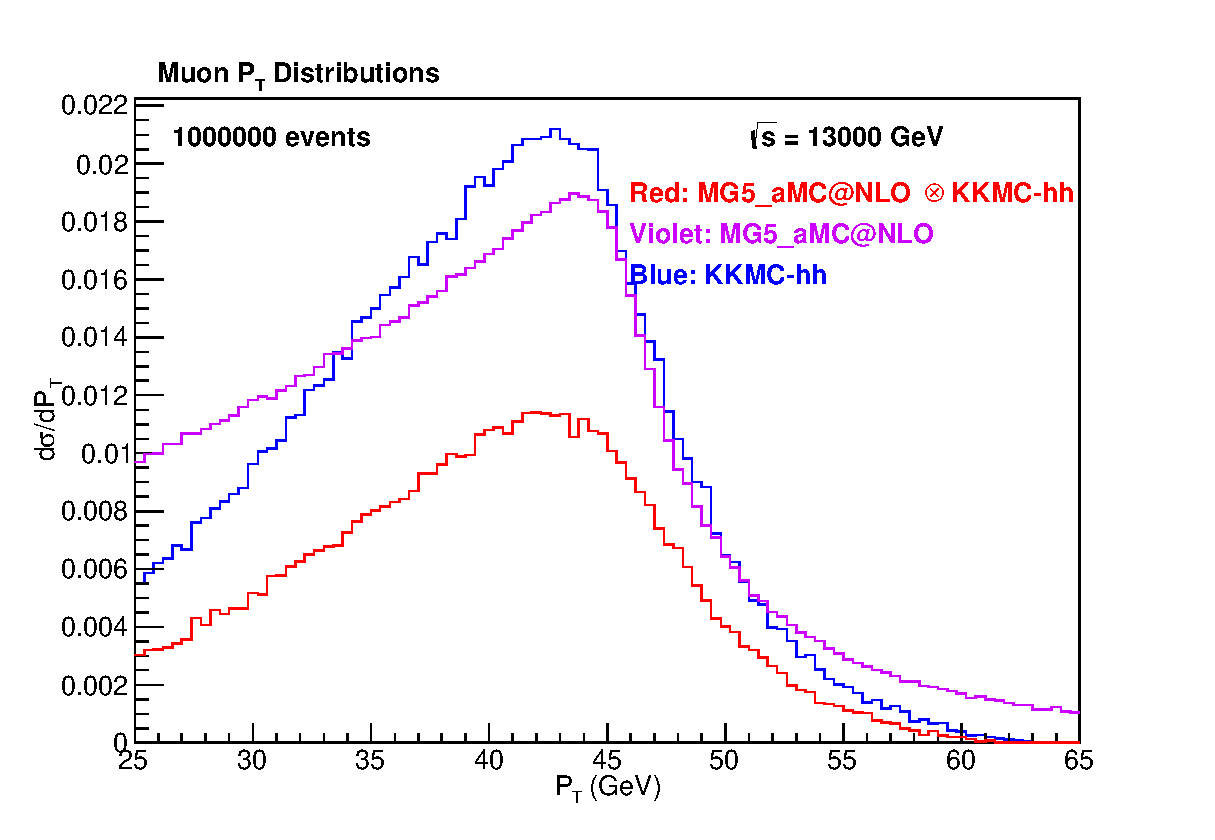
\includegraphics[scale=0.65]{PTL.eps}
		\caption{ Muon transverse momentum distributions for KKMC-hh (blue), MG5\textunderscore aMC@NLO (violet) and MG5\textunderscore aMC@NLO interfaced with KKMC-hh (red) with the cuts specified in the text. }
	\end{center}
\end{figure}

The next quantity we compared is the muon pseudorapidity distribution. The pseudorapidity $\eta$ is a spatial coordinate describing the angle of a particle relative to the beam axis, commonly used in the experimental particle physics. It is defined as 
\begin{equation}
\eta=\log\left(\tan\frac{\theta}{2}\right),
\end{equation} 
where the angle $\theta$ is angle between the particle three-momentum $\vec{p}$ and the positive direction of the beam axis. The pseudorapidity can also be expressed in terms of three-momentum:
\begin{equation}
\eta\equiv\frac{1}{2}\log\left(\frac{|p|+p_L}{|p|-p_L}\right),
\end{equation}
where $p_L$ is the component of the momentum along the beam axis, namely, the longitudinal momentum. From Figure 8.2, we find that interfacing MG5\textunderscore aMC@\newline
NLO with KKMC-hh results an apparent enhancement on the muon pseudorapidity distribution compared with that derived from MG5\textunderscore aMC@NLO.
\begin{figure}
	\begin{center}
		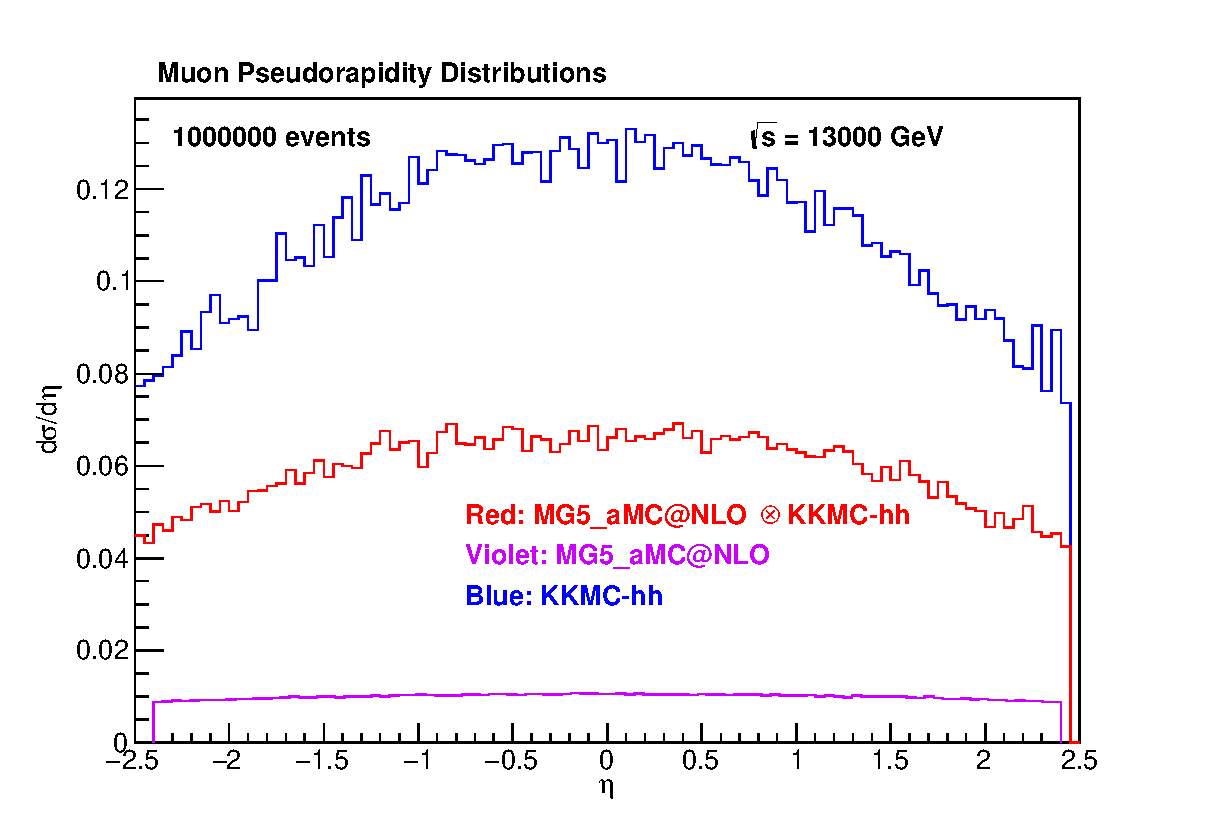
\includegraphics[scale=0.65]{ETA.eps}
		\caption{ Muon pseudorapidity distributions for KKMC-hh (blue), MG5\textunderscore aMC@NLO (violet) and MG5\textunderscore aMC@NLO interfaced with KKMC-hh (red) with the cuts specified in the text. }
	\end{center}
	\end{figure}

We compared not only quantities of the single lepton but those of lepton pairs as well. The dimuon transverse momentum distributions obtained by these three approaches are given in the Figure 8.3. As we can see, the differential cross section calculated by MG5\textunderscore aMC@NLO interfaced with KKMC-hh is larger than that obtained by MG5\textunderscore aMC@NLO only, and the enhancement is from the EW corrections calculated by KKMC-hh. 

And the Figure 8.4 described the dimuon invariant mass distributions. By comparing the dimuon invariant mass distribution derived from MG5\textunderscore aMC@NLO interfaced with KKMC-hh with that from MG5\textunderscore aMC@NLO only, we find there is also an enhancement that is due to the EW corrections provided by KKMC-hh. Besides, we see the resonance peaks near $91\text{ GeV}$ derived from these three generators.
\begin{figure}
	\begin{center}
		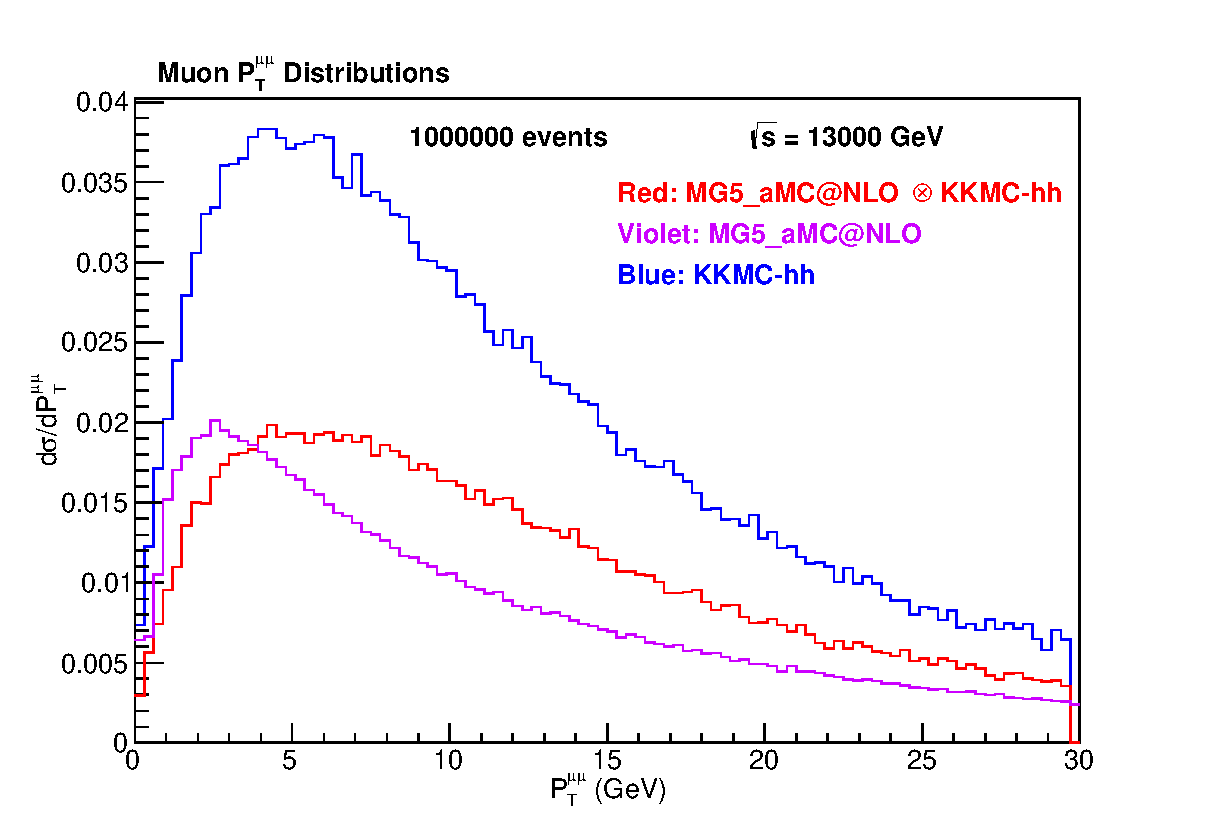
\includegraphics[scale=0.65]{PTLL.eps}
		\caption{ Dimuon transverse momentum distributions for KKMC-hh (blue), MG5\textunderscore aMC@NLO (violet) and MG5\textunderscore aMC@NLO interfaced with KKMC-hh (red) with the cuts specified in the text.  }
	\end{center}
\end{figure}

Finally, let us see the dimuon rapidity distributions in the Figure 8.5. The rapidity is defined as 
\begin{equation}
y\equiv\frac{1}{2}\log\left(\frac{E+p_L}{E-p_L}\right).
\end{equation}
We see that MG5\textunderscore aMC@NLO interfaced with KKMC-hh amplified the dimuon rapidity distribution obtained by MG5\textunderscore aMC@NLO only. The amplification can be viewed as a consequence of the EW corrections.


\begin{figure}
	\begin{center}
		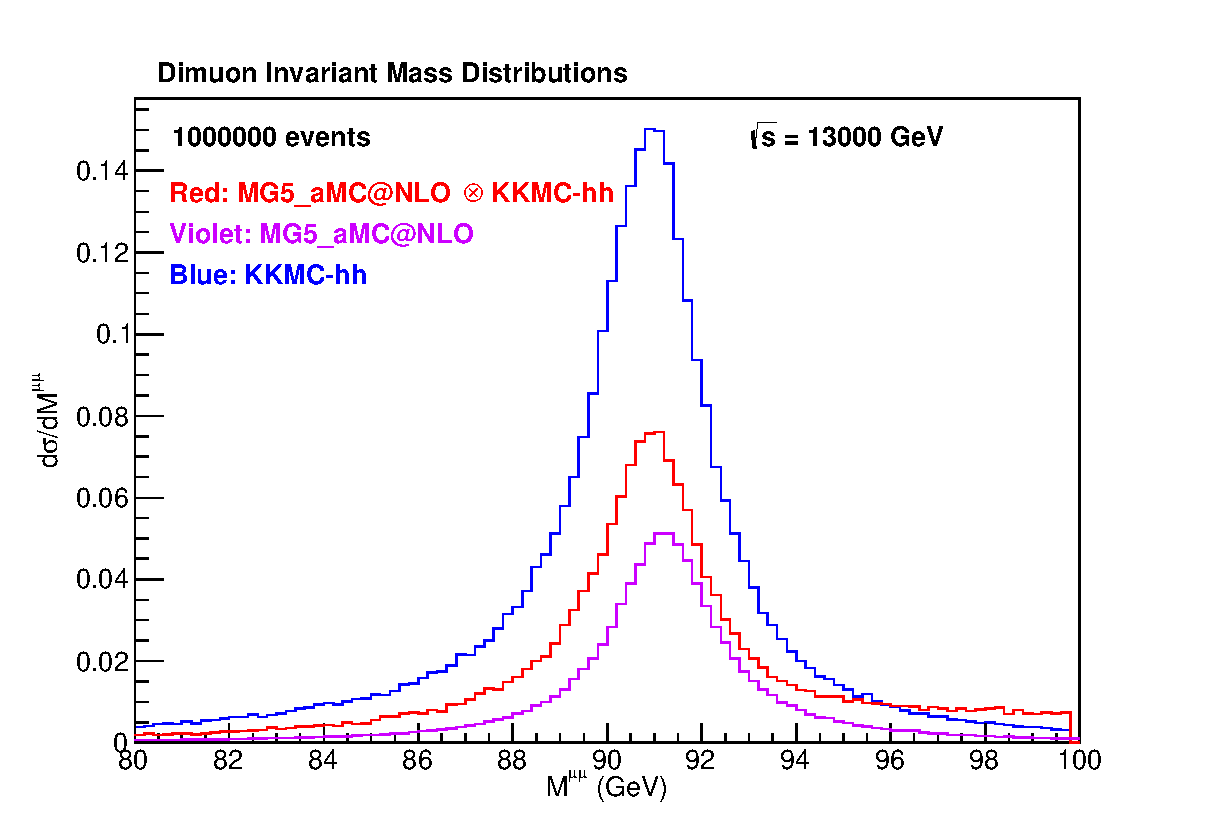
\includegraphics[scale=0.65]{MLL.eps}
		\caption{ Dimuon invariant mass distributions for KKMC-hh (blue), MG5\textunderscore aMC@NLO (violet) and MG5\textunderscore aMC@NLO interfaced with KKMC-hh (red) with the cuts specified in the text. }
	\end{center}
\end{figure} 

In sum, we exhibited the comparisons of the results obtained by MG5\textunderscore aMC@\newline NLO$\otimes$KKMC-hh, MG5\textunderscore aMC@NLO and KKMC-hh. We find that MG5\textunderscore aMC@NLO interfaced with KKMC-hh would enhance the results obtained by MG5\textunderscore aMC@NLO only and the enhancement is due to the EW corrections derived from KKMC-hh.

\begin{figure}
	\begin{center}
		\includegraphics[scale=0.65]{Y.eps}
		\caption{ Dimuon radipity distributions for KKMC-hh (blue), MG5\textunderscore aMC@NLO (violet) and MG5\textunderscore aMC@NLO interfaced with KKMC-hh (red) with the cuts specified in the text. }
	\end{center}
\end{figure}